\documentclass[12pt,letterpaper]{beamer}
\usetheme{Copenhagen}
\usecolortheme{seahorse}
\setbeamertemplate{section in toc}{\inserttocsection}

\usepackage[utf8]{inputenc}
\usepackage{amsmath}
\usepackage{amsfonts}
\usepackage{amssymb}
\usepackage{graphicx}
\graphicspath{ {./images/} }
\usepackage{multirow}
\usepackage{hyperref}
\hypersetup{
    colorlinks=true,
    linkcolor=blue,
    filecolor=magenta,      
    urlcolor=cyan,
    pdftitle={Overleaf Example},
    pdfpagemode=FullScreen,
}
\title[Robotics I]
{ENGR 3421: ROBOTICS I}
\subtitle{Introduction to Linux}

\author[Zhang, Lin]
{Dr. Lin Zhang}
\institute[UCA] % (optional)
{
  Department of Physics and Astronomy\\
  University of Central Arkansas
}
\date[Robotics1 2021] % (optional)
{September 7, 2021}
\logo{
\includegraphics[height=1cm]{../images/uca_bear_logo.png}}


%End of title page configuration block
%------------------------------------------------------------

%------------------------------------------------------------
%The next block of commands puts the table of contents at the beginning of each section and highlights the current section:

\AtBeginSection[]
{
  \begin{frame}
    \frametitle{outline}
    \tableofcontents[currentsection]
  \end{frame}
}
%------------------------------------------------------------

\begin{document}

%The next statement creates the title page.
\frame{\titlepage}

%---------------------------------------------------------
%This block of code is for the table of contents after the title page
\begin{frame}
\frametitle{Outline}
\tableofcontents
\end{frame}
%---------------------------------------------------------

\section{Story of Linux}

\begin{frame}{Story of Linux}
    {\centering
        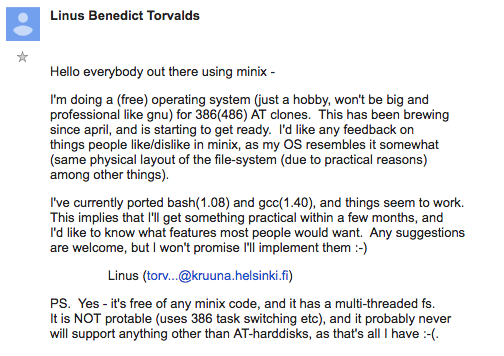
\includegraphics[width=0.8\linewidth]{linus_torvald_first_linux_email}
    }
\end{frame}

\begin{frame}{Linux Distros}
    Distro is a complete operating system based on the Linux kernel that contains a bunch of packages and libraries.
    \begin{itemize} 
        \item Debian(for home users)
        \item Redhat(for enterprises)
        \item Slackware
        \item Android
    \end{itemize} 
\end{frame}

\section{Linux Command Line}
\begin{frame}{Linux Command Line}
    The Linux command line is a text interface to your computer.
\end{frame}

\begin{frame}{HC-SR04 - No Object Detected}
    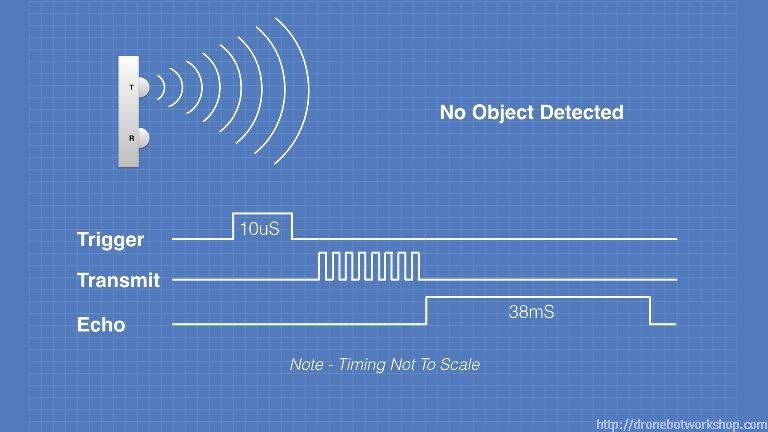
\includegraphics[width=.95\linewidth]{no_object}
\end{frame}

\begin{frame}{HC-SR04 - Object Detected}
    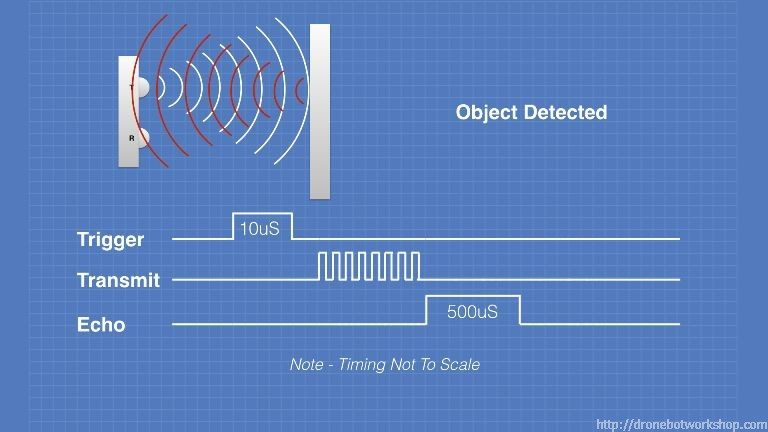
\includegraphics[width=.95\linewidth]{object_detect}
    \begin{equation*}
        distance = \frac{Speed \times Time}{2} = 0.034cm/{\mu}s \times 500{\mu}s \times 0.5
    \end{equation*}
\end{frame}

\begin{frame}{HC-SR04 Workflow}

    {\scriptsize
        \begin{enumerate}
            \item A 5 volt pulse of at least 10 $\mu$S (10 microseconds) in duration is applied to the Trigger pin.
            \item The HC-SR04 responds by transmitting a burst of eight pulses at 40 KHz. This 8-pulse pattern makes the “ultrasonic signature” from the device unique, allowing the receiver to discriminate between the transmitted pattern and the ultrasonic background noise.
            \item The eight ultrasonic pulses travel through the air away from the transmitter. Meanwhile the Echo pin goes high to start forming the beginning of the echo-back signal.
            \item If the pulse in NOT reflected back then the Echo signal will timeout after 38 mS (38 milliseconds) and return low. This produces a 38 mS pulse that indicates no obstruction within the range of the sensor.
            \item If the pulse IS reflected back the Echo pin goes low when the signal is received.  This produces a pulse whose width varies between 150 uS to 25 mS, depending upon the time it took for the signal to be received.
            \item The width of the received pulse is used to calculate the distance to the reflected object. Remember that the pulse indicates the time it took for the signal to be sent out and reflected back so to get the distance you’ll need to divide your result in half.
        \end{enumerate}
    }
\end{frame}

\begin{frame}{HC-SR04 Limitations}

    {\small
        \begin{itemize}
            \item Object too far.
            \item Object too small.
            \item Object with soft irregular surface.
            \item Effect of temperature and humidity. A more accurate distance calculation: $Speed(m/s) = 331.4 + (0.606 * Temp) + (0.0124 * Humidity)$
            \item Ultrasound may annoying to animals. Please consider your furry friends (Check the \href{https://en.wikipedia.org/wiki/Hearing_range}{hearing range list}).
        \end{itemize}
    }
\end{frame}

\begin{frame}{Voltage Divider}
    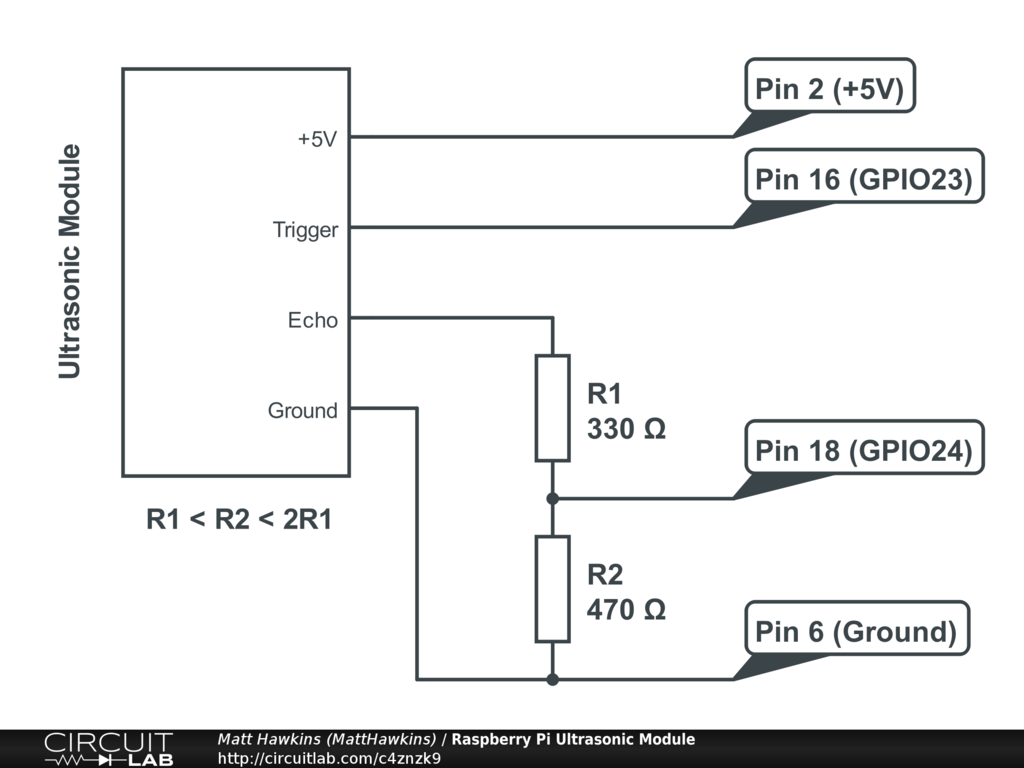
\includegraphics[width=.95\linewidth]{voltage_divider}
\end{frame}



\end{document}

